\chapter{Versuchsaufbau und -ablauf}\label{Kap3}

Das folgende Kapitel beschreibt Versuchsaufbau und -durchf"uhrung sowie Ziele der Messung, von der Erkenntnisse "uber das Skalierungsverhalten eines RPi-Clusters unter der Arbeitslast der ausgew"ahlten HPC-Benchmarks erwartet werden. 

\section{Zielsetzung}\label{Ziel}

F"ur das Skalierungsverhalten des Bramble unter der Workload von Linpack und STREAM werden wie in Kap. \ref{Kapitel 2} beschrieben zwei Ma\ss zahlen betrachtet: Performance und Energieverbrauch.

Die augew"ahlten Benchmarks werden auf n--1 RPi-Knoten des Bramble mit n=19 RPi-Nodes ausgef"uhrt (vgl. Kap. \ref{Versuchsaufbau}). Alle Messungen werden zweimal durchgef"uhrt: Mit Stromanschluss der nicht beteiligten RPi-Nodes und ohne. F"ur beide Benchmarks werden zwei Ergebnisparameter betrachtet: Ausf"uhrungsrate in GFLOPs und Ausf"uhrungszeit in s f"ur HPLinpack, Ausf"uhrungsrate in MB/s und durchschnittliche Ausf"uhrungszeit in s f"ur STREAM. Die Ergebnisse der Messreihen werden anschlie\ss end gegen"ubergestellt (vgl. Kap. \ref{Ergebnisse}). 

\section{Aufbau und Art der Messung}\label{Aufbau}

Hier stellen sich zwei grunds"atzliche Fragen: Welcher Art ist die Messung und welche Voraussetzungen m"ussen hierf"ur erf"ullt sein? 

Die Performance wird pro Benchmark durch zwei Ergebnisparameter ermittelt. Zwei Messreihen werden durchgef"uhrt: Bramble mit n--1 RPi-Knoten aktiv/19 RPi-Knoten angeschaltet, Bramble mit n--1 RPi-Knoten aktiv/n RPi-Knoten angeschaltet. 
% TODO: evtl. bessere Einleitung/Herleitung 
F"ur den Versuchsaufbau sind folgende Aspekte von Bedeutung: M"ogliche Modifikationen der RPi-Knoten (Hardware, Betriebssystem-Konfiguration), Zeitsynchronisation der RPi-Knoten, Skalierung der Messung auf n--1 RPi-Knoten, automatisierte Durchf"uhrung der Messung auf 19--n RPi-Knoten sowie Einlesen der Messwerte in eine geeignete Datenstruktur. 

\subsection{Versuchsaufbau Ri-Einzelrechner}\label{RPi-Versuchsaufbau}

Viele Nutzer stellen sich nach Inbetriebnahme eines RPi-Einzelrechners die Frage nach Swap-Speicher und "Ubertakten (vgl. \cite{pow12}). Beides liegt nahe, da das Modell B des RPi nur "uber 512 MB Arbeitsspeicher verf"ugt. Die CPU-Leistung ist mit 700 MHz ebenfalls eher niedrig. 

Im Praxisbetrieb wurde gezeigt, dass ein "Ubertakten der CPU auf bis zu 1 GHz gefahrlos m"oglich ist. Bei den hier verwendeten RPis wurde darauf verzichtet, da es wenig zielf"uhrend erscheint, die Komponente zu manipulieren, deren Performance man durch Benchmarking evaluieren m"ochte\footnote{F"ur eine zuk"unftige Untersuchung w"are es interessant zu ermitteln, ob man den relativ hohen Stromverbrauch des Bramble bei Niedriglast (vgl. \cite{kli13}) durch Untertakten der einzelnen CPUs senken kann (vgl. \ref{Kap5}).} Allerdings gibt es bereits Ergebnisse f"ur Linpack 100 und Whetstone bei auf einem RPi-Einzelrechner bei "Ubertakten der CPU auf 1 MHz (vgl. \url{http://www.roylongbottom.org.uk/Raspberry\%20Pi\%20Benchmarks.htm}).

Zur Allokierung von Swap-Speicher auf dem RPi gibt es grunds"atzlich drei M"oglichkeiten: Swap-Datei, Swap-Partition oder zRAM. 

Das Betriebssystem Raspbian verwendet standardm"a\ss ig eine Swap-Datei \texttt{/var/swap} auf der SD-Karte (vgl. \url{http://raspberrypi.stackexchange.com/questions/70/how-to-set-up-swap-space}). Hierbei zeigen sich Probleme: Erstens k"onnen st"andige Schreibzugriffe auf Dauer die SD-Karte besch"adigen. Zweitens sind Schreibzugriffe darauf sehr langsam, was die Performance des Systems bei hoher Arbeitsspeicherlast beeintr"achtigen kann (vgl. \cite{pow12}). 

Das gilt auch f"ur die Allokierung einer auf Unix-Systemen "ublicherweise genutzten Swap-Partition, weswegen diese M"oglichkeit in der Praxis keine Rolle spielt. 

Eine weitere M"oglichkeit des Swapping ist die Verwendung von zRAM. Hierbei wird ein Teil des Arbeitsspeichers komprimiert und als Swap Space genutzt. Hierbei werden keine Zugriffe auf die SD-Karte notwendig (vgl. \cite{pow12}). 

% Die Swap-Datei kann mit dem Befehl \texttt{sudo update-rc.d dphys-swapfile remove} deaktiviert werden. 
Auf dem Bramble-Server war kein Swap-Speicher allokiert worden (vgl. \cite{kli13}). Trotz der beschriebenen Schwierigkeiten wird auf den RPi-Knoten ein gro\ss er Teil des Speichers auf den SD-Karten als Swap-Speicher genutzt, um die Nutzung von Programmen mit mehr Speicherbedarf zu erm"oglichen und das Netzwerk durch das Cachen h"aufig verwendeter Dateien zu entlasten (vgl. \cite{kli13}).  

\subsection{Versuchsaufbau Bramble}\label{Bramble-Versuchsaufbau}

Das Komponentendiagramm \ref{fig:Komponentendiagramm} zeigt den Versuchsaufbau pro Messreihe auf dem Bramble, der als \textit{ExperimentSuite} bezeichnet wird. Es enth"alt die systemkritischen Elemente des Versuchsaufbaus: Stromversorgung und Netzanschluss des Bramble sowie das Strommessger"at als physische Komponenten und die MySQL-Datenbank \texttt{rpiWerte} als logische Komponente. 
\begin{figure}[htb]
  \centering
  \includegraphics[width=\textwidth]{komponentendiagramm1.pdf}\\ 
  \caption{Komponentendiagramm des Versuchsaufbaus.}
  \label{fig:Komponentendiagramm}		
\end{figure}

\subsubsection{Modifikationen der RPi-Nodes}

Betriebssystem und Filesystem des Bramble wurden so "ubernommen wie bei Beginn der Untersuchung zur Verf"ugung gestellt: Die CPUs der RPi-Nodes sind nicht "ubertaktet und der Bramble-Server \texttt{careme} nutzt keinen Swap Space. Bei den RPi-Nodes war allerdings ein gro\ss er Teil der SD-Karten als Swap Space allokiert worden\footnote{Vgl. \cite{kli13}.}. Im Praxisbetrieb zeigten sich jedoch rasch Schwierigkeiten, die Anpassungen in OS-Konfiguration und Hardware erforderlich machten. Folgende Fehlerf"alle waren am h"aufigsten: 
\begin{enumerate}
	\item \textbf{Defekte Hardware (Mini-USB-Kabel)}\\
Einige Mini-USB-Kabel waren bereits zu Beginn der Untersuchung defekt oder hatten einen Wackelkontakt. Sie mussten durch funktionsf"ahige Kabel ersetzt werden. 
	\item \textbf{RPi-Node nicht erreichbar (\texttt{ping})}\\
H"aufig reagierte ein RPi-Node nicht auf ein \texttt{ping} von einem RPi-Node oder von \texttt{careme} aus (Fehlermeldung \texttt{Destination Host Unreachable}), obwohl die Status-LEDs aktiv waren. Als einzige L"osung erwies sich Ziehen und Wiedereinstecken des Mini-USB-Kabels; war das nicht erfolgreich, musste das Vorgehen mit dem Netzwerkkabel wiederholt werden (das Netzwerkkabel allein reicht nicht aus). Danach war der Host i.d.R. wieder mit \texttt{ping} erreichbar. 
	\item \textbf{RPi-Node nicht erreichbar (SSH)}\\ 
Hier traten drei Fehlerf"alle auf: Am h"aufigsten war die Fehlermeldung \texttt{No route to host} beim Versuch, von \texttt{careme} oder einem anderen RPi-Node aus eine SSH-Verbindung zum Zielhost herzustellen. Die einzige L"osung ist Ziehen und wieder Einstecken des Netzwerkkabels. Nach einigen Minuten ist der Host i.d.R. wieder erreichbar. 

Ein weiterer Fehlerfall war ein "uberraschender Passwortprompt f"ur \texttt{root} beim Versuch, eine SSH-Verbindung zu einem RPi-Node zu einem anderen RPi-Zielnode aufzubauen. Dieses Problem lie\ss sich durch Eintragen des RSA Public Key von 
\texttt{root} in die Datei \texttt{\textasciitilde/.ssh/authorized\_keys} auf dem Zielhost l"osen. 

Seltener trat die Fehlermeldung \texttt{WARNING: REMOTE HOST IDENTIFICATION HAS CHAN\-GED!} auf. Dies konnte durch Korrektur des RSA Public Key des Anfragehosts in der Datei \texttt{\textasciitilde/.ssh/known\_hosts} auf dem Zielhost gel"ost werden. 
	\item \textbf{Geshartes Verzeichnis nicht gemountet}\\
Beim Neustart eines RPi-Nodes oder des gesamten Clusters wurde h"aufig das gesharte Verzeichnis nicht gemountet, was zu Fehlermeldungen wie \texttt{-bash: /srv/libraries/ etc/.sharedprofile: No such file or directory} f"uhrte und sich durch Mounten des Verzeichnisses mit \texttt{mount /srv} beheben lie\ss .
	\item \textbf{bash-Befehle werden nicht erkannt}\\
Aus unklaren Gr"unden wurden manchmal von einzelnen RPi-Nodes h"aufig verwendete bash-Befehle nicht mehr erkannt, was sich an Fehlermeldungen wie \texttt{mpiexec: command not found} zeigt. Latenzen beim Zugriff auf den gemeinsamen Speicherbereich k"onnten der Grund hierf"ur sein, da sich ein Logout und erneuter Login auf dem betreffenden RPi-Node als einzige L"osung erwies. 
\end{enumerate}

\subsubsection{Zeitsynchronisation der RPi-Nodes} 

Der RPi-Einzelrechner besitzt aus Kostengr"unden keine Systemuhr (vgl. \cite{sch13}), sondern synchronisiert sich beim Booten gegen einen NTP-Server im Internet. F"ur die parallele Ausf"uhrung eines Programms auf mehreren Rechnerkernen ist die Zeitsynchronisation der RPi-Knoten und des Servers essentiell. Auf dem Bramble-Server gibt es daher einen OpenNTP-Server, gegen den sich die RPi-Knoten synchronisieren (vgl. \cite{kli13}). 

\subsubsection{Skalierung der Messung auf 19--n RPi-Nodes} 

Das folgende Aktivit"atsdiagramm zeigt, welche Schritte aus Benutzersicht f"ur die Durchf"uhr\-ung einer ExperimentSuite, d.h. der Ausf"uhrung eines Benchmarks auf einer gew"ahlten Anzahl von aktiver und powered RPi-Nodes erforderlich sind. Es wird mit n=19 RPi-Nodes begonnen und einmal "uber alle Nodes von 20--1 (ohne den Ausf"uhrungsknoten \texttt{pi03}) iteriert. Danach wird die zweite Messung durchgef"uhrt, wobei nach jedem Iterationsschritt der nicht mehr ben"otigte RPi-Node abgeschaltet wird. Jede Iteration der Benchmark-Ausf"uhrung l"auft prinzipell gleich ab, w"ahrend am Anfang und am Ende spezielle Vorkehrungen zu treffen sind. 
\begin{figure}[htb]
  \centering
  \includegraphics[scale=0.5]{aktivitaetsdiagramm1.pdf}\\ 
  \caption{Aktivit"atsdiagramm der ExperimentSuite.}
  \label{fig:Aktivitaetsdiagramm}
\end{figure}

\subsubsection{Automatisierte Durchf"uhrung der Messung auf 19--n RPi-Nodes} 

Die automatisierte Durchf"uhrung der Messung erfolgt durch Shellskripte. Sie werden im gesharten Verzeichnis abgelegt und k"onnen von \texttt{pi03} oder einem anderen Ausf"uhrungsknoten aus gestartet werden. Folgende Schritte werden durch die Skripte realisiert: 

\begin{enumerate}
	\item Erstellen eines Machinefile zur Verteilung der Workload auf n RPi-Nodes, ggf. L"oschen des alten.
	\item Mounten des gesharten Verzeichnisses auf allen RPis. 
	\item Navigation ins Arbeitsverzeichnis der Experimentsuite. 
	\item Iteration "uber n ausgew"ahlte Benchmarks: 
	\begin{enumerate}
		\item Erstellen der Logfiles. 
		\item Iteration "uber n RPi-Nodes:
		\begin{enumerate}
			\item Einrichten der Datenbank. 
			\item Verteilte Ausf"uhrung des Benchmarks auf n RPi-Nodes. 
			\item Loggen der Ergebnisdaten. 
		\end{enumerate}
		\item Iteration "uber n RPi-Nodes: 
		\begin{enumerate}
			\item Einrichten der Datenbank.
			\item Verteilte Ausf"uhrung des Benchmarks auf n RPi-Nodes. 
			\item Shutdown von RPi-Node n. 
			\item Loggen der Egebnisdaten.   
		\end{enumerate}
		\item Parsen der Logfiles f"ur die Datenbank-Eingabe. 
		\item Schreiben der Messergebnisse in die Datenbank. 
	\end{enumerate}
\end{enumerate}
\noindent
Dazu wurden drei Shellskripte \texttt{startBenchmarks.sh} (Schritte 1--3), \texttt{STREAM.sh} und \texttt{hpl-2.1.sh} (Schritt 4 f"ur den jeweiligen Benchmark) erstellt. Der Quellcode findet sich in \mbox{Kap. \ref{skripte}}.

\subsubsection{Einlesen der Messwerte in eine geeignete Datenstruktur}

Schlie\ss lich stellt sich die Frage, wo und in welcher Form die Ergebnisdaten zweckm"assigerweise abgelegt werden. Die Entscheidung fiel zu Gunsten einer MySQL-Datenbank auf \texttt{careme}. Sie orientiert sich an einem vorgegebenen Datenbankschema, das die Bramble-ExperimentSuites in einen gr"o\ss eren Versuchsaufbau integriert. W"ahrend der praktischen Arbeit wurde das Schema schrittweise an die tats"achlichen Erfordernisse angepasst. Z.B. wurde f"ur jedes ausgef"uhrte Teilmodul eines Benchmarks ein Parameter definiert, der Unix-Timestamp seines Ausf"uhrungsendes ermittelt und zusammen mit dem jeweiligen Messwert in die Datenbank eingelesen.

Um dem gew"ahlten Datenbankschema gerecht zu werden, mussten neben der Tabelle mit den Messergebnissen weitere Tabellen bef"ullt und "uber eine N2M-Tabelle verkn"upft werden (vlg. \ref{fig:Aktivitaetsdiagramm}, "`Datenbank vorbereiten"'): 
\begin{enumerate}
	\item Benennung und Beschreibung des Benchmarks 
	\item Benennung und Beschreibung des Versuchsaufbaus 
	\item Konfiguration des Versuchsaufbaus 
\end{enumerate} 
Im ersten Schritt werden die statischen Konfigurationen f"ur STREAM und HPLinpack festgelegt, was durch zwei weitere Shellskripte \texttt{loadGeneratorConfigHpl.sh} und \texttt{loadGenerator\-ConfigStream.sh} (vgl. Kap. \ref{skripte}) realisiert wurde. Die dynamischen Schritte pro ExperimentSuite (Benennung, Beschreibung und Konfiguration des Versuchsaufbaus, Einlesen der Messwerte und Verkn"upfung von ExperimentSuite mit Benchmark-Konfiguration) wurden in die Ausf"uhrungsskripte der Benchmarks integriert. 

\section{Ergebnisse}\label{Ergebnisse}

Der n"achste Abschnitt pr"asentiert die Untersuchungsergebnisse mit Schwerpunkt auf dem Bramble. F"ur die Durchf"uhrung standen auf Grund der oben beschriebenen Probleme nur 17 RPi-Nodes zuverl"assig zur Verf"ugung. Zur besseren Lesbarkeit der Ergebnisse wurde entschieden, beide Benchmarks auf gleich vielen RPi-Nodes auszuf"uhren. Da HPLinpack mindestens vier Prozessoren bzw. Prozesse ben"otigt, wurde die Anzahl der Prozessoren f"ur STREAM hieran angepasst. Beide Benchmarks wurden demnach auf n=16 RPi-Nodes ausgef"uhrt, \texttt{pi03} dient als Ausf"uhr\-ungsknoten und wird in der Messung nicht ber"ucksichtigt.

\subsection{RPi-Einzelrechner: Linpack 100, Whetstone und STREAM}\label{rpi-ergebnisse}

Bei der Ausf"uhrung von Linpack 100, Whetstone und STREAM in den ausgew"ahlten Implementierungen erreichte der RPi-Einzelrechner folgende Ergebnisse: 

\begin{enumerate}
	\item \textbf{Linpack 100} 
	\begin{itemize}
		\item \textbf{Ausf"uhrungsrate:} 41.31 MFLOPS = 0.04131 GFLOPS
	\end{itemize}
	\item \textbf{Whetstone} 
	\begin{itemize}
		\item \textbf{Ausf"uhrungsrate:} 255.154 MWIPS
		\item \textbf{Ausf"uhrungszeit:} 10.190 s  
	\end{itemize}
	\item \textbf{STREAM} 
	\begin{itemize}
		\item \textbf{Ausf"uhrungsrate:}
		\begin{enumerate}
			\item COPY: 274.4. MB/s
			\item SCALE: 209.3 MB/s
			\item ADD: 287.2 MB/s
			\item TRIAD: 271.1 MB/s
		\end{enumerate}					 
		\item \textbf{Ausf"uhrungszeit:}
		\begin{enumerate}
			\item COPY: 0.586838 s
			\item SCALE: 0.766437 s
			\item ADD: 0.838107 s
			\item TRIAD: 0.886793 s
		\end{enumerate}
	\end{itemize}
\end{enumerate} 
Detaillierte Ergebnisdateien finden sich im Anhang (vgl. Kap. \ref{rpi-anhang}). 
 
\subsection{Bramble: HPLinpack}\label{Ergebnisse-HPL}

Die folgenden Diagramme zeigen die Ergebnisse f"ur HPLinpack auf dem Bramble mit zwei Ausgabeparametern: Time to Completion und CPU-Performance in MFLOPS, jeweils skaliert auf 16--4 RPi-Nodes. Diagramme \ref{fig:hpl1} und \ref{fig:hpl2} zeigen die Ergebnisse f"ur n RPi-Nodes aktiv/16 RPi-Nodes powered (d.h. alle). Diagramme \ref{fig:hpl3} und \ref{fig:hpl4} zeigen das Verhalten bei n RPis aktiv/n RPis powered.
\enlargethispage*{2cm}
\begin{figure}[htb]
  \centering
  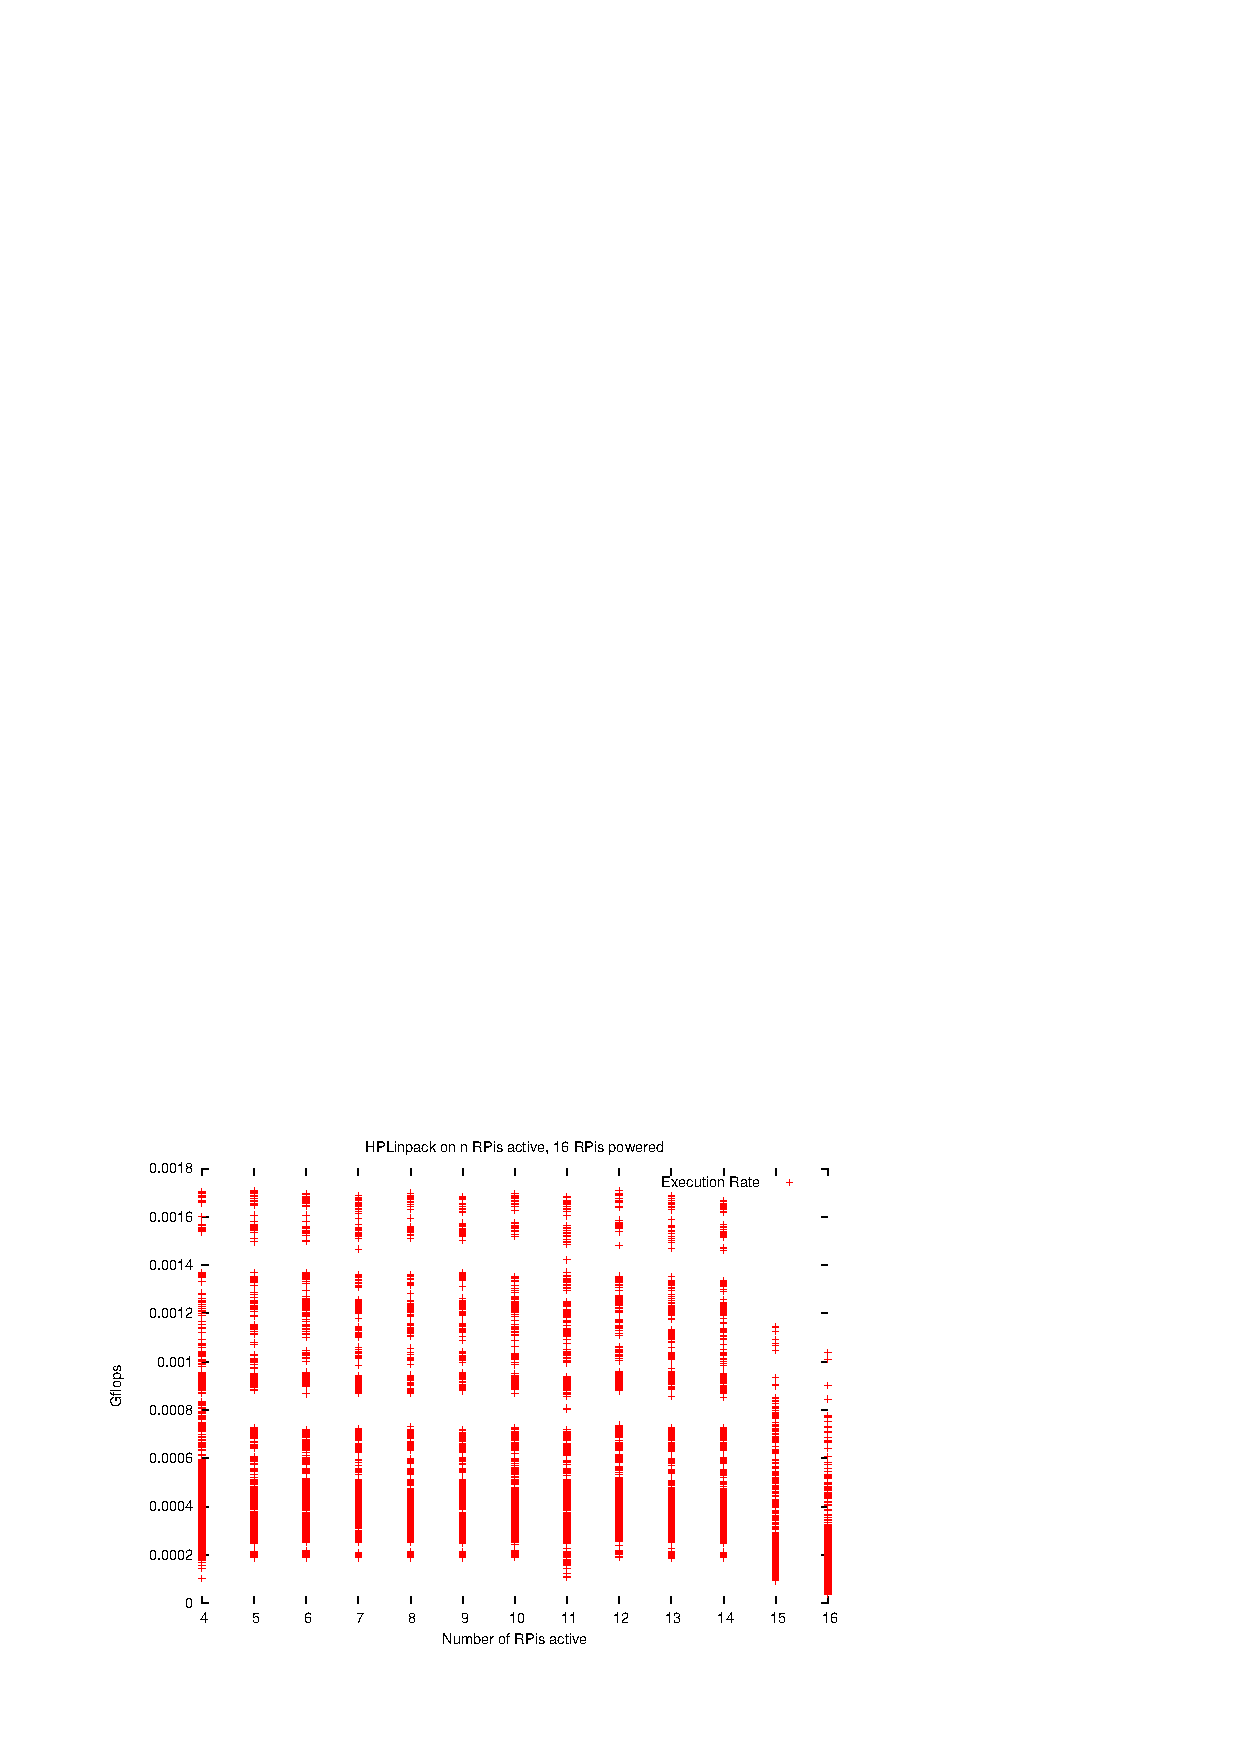
\includegraphics[scale=0.8]{hpl1.pdf}\\ 
  \caption{Ausf"uhrungsrate in GFLOPS f"ur HPLinpack auf n RPi-Nodes aktiv/16 RPi-Nodes powered.}
  \label{fig:hpl1}		
\end{figure}
\begin{figure}[h!]
  \centering
  \includegraphics[scale=0.8]{hpl2.pdf}\\ 
  \caption{Ausf"uhrungszeit in s f"ur HPLinpack auf n RPi-Nodes aktiv/16 RPi-Nodes powered.}
  \label{fig:hpl2}		
\end{figure}
\begin{figure}[htb]
  \centering
  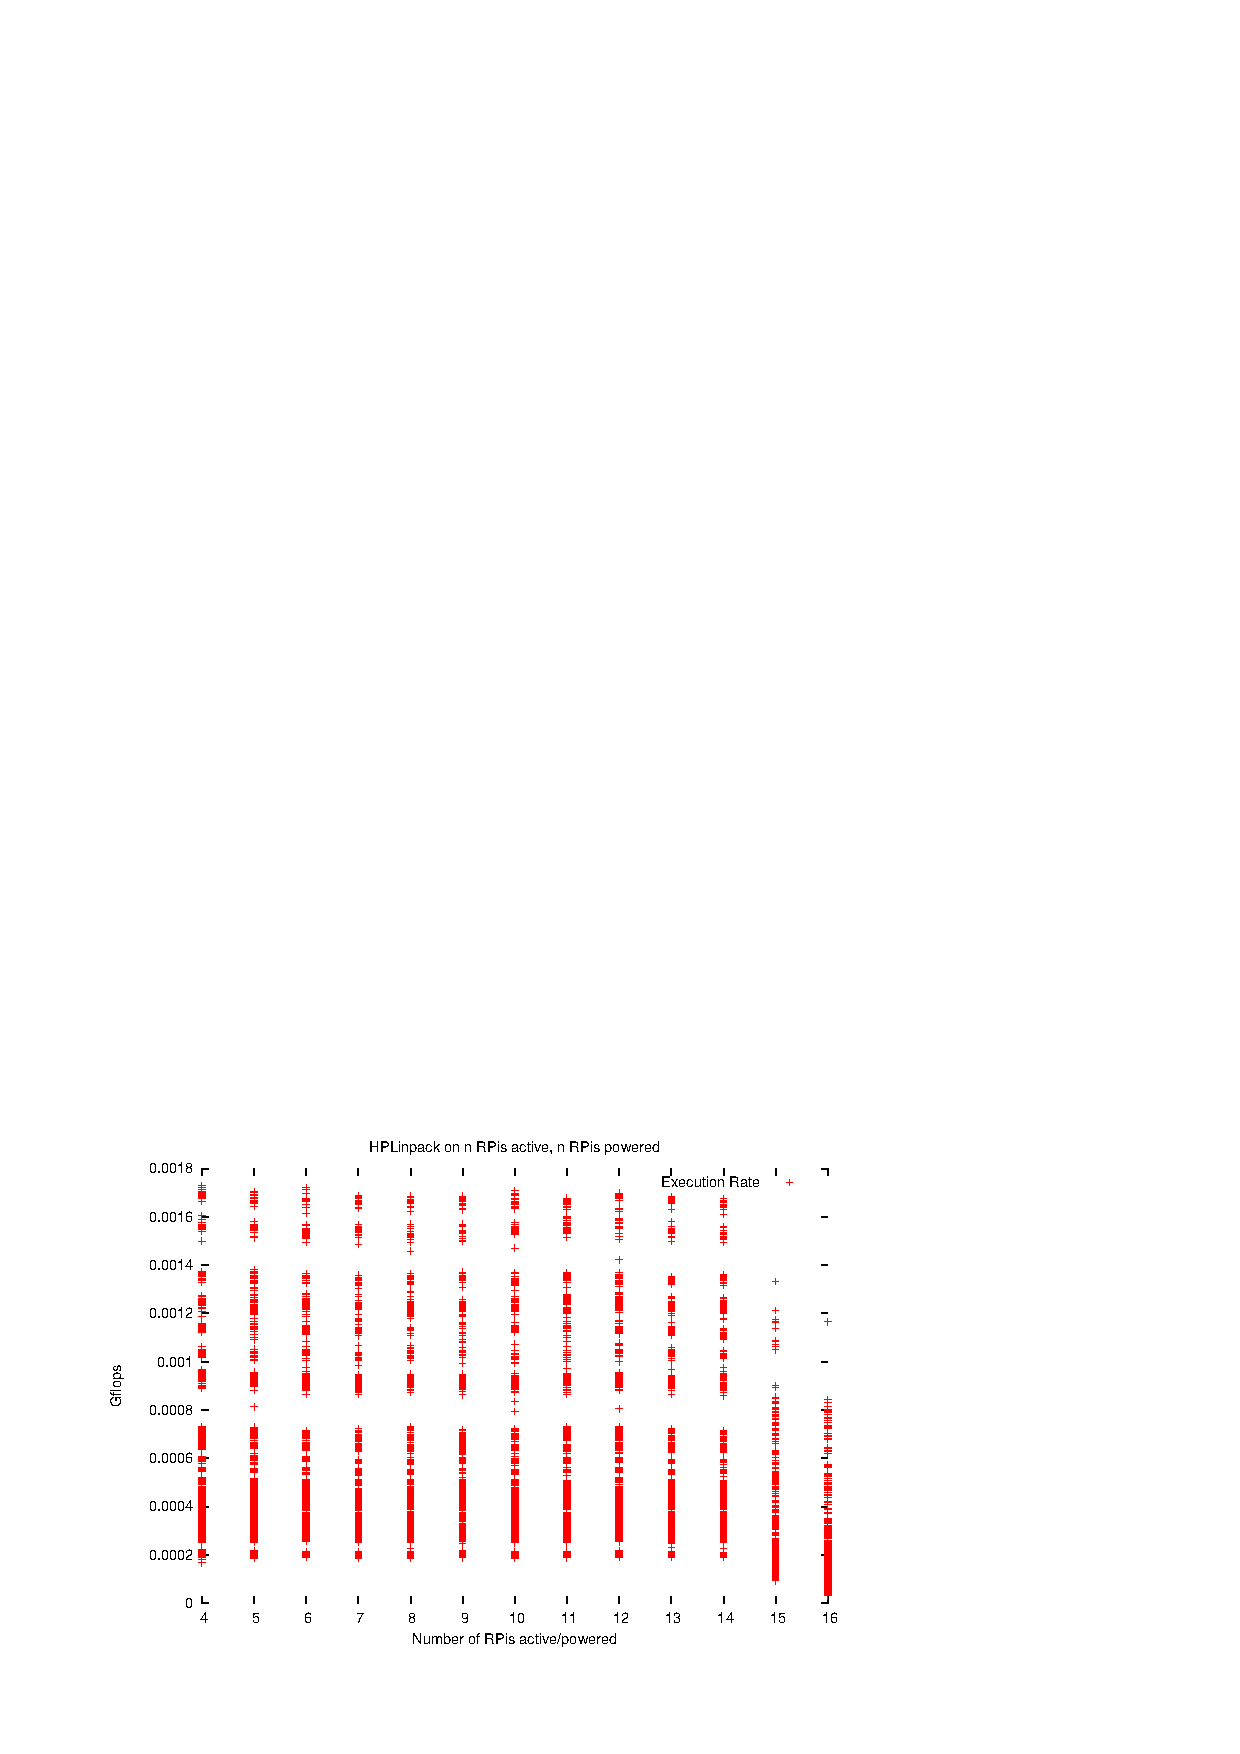
\includegraphics[scale=0.8]{hpl3.pdf}\\ 
  \caption{Ausf"uhrungsrate in GFLOPS f"ur HPLinpack auf n RPi-Nodes aktiv/n RPi-Nodes powered.}
  \label{fig:hpl3}		
\end{figure}
\begin{figure}[h!]
  \centering
  \includegraphics[scale=0.8]{hpl4.pdf}\\ 
  \caption{Ausf"uhrungszeit in s f"ur HPLinpack auf n RPi-Nodes aktiv/n RPi-Nodes powered.}
  \label{fig:hpl4}		
\end{figure}

\newpage
\subsection{Bramble: STREAM}\label{Ergebnisse-Stream}
Die folgenden Diagramme zeigen die Ergebnisse von STREAM auf dem Bramble f"ur die Module Copy, Scale, Add und Triad, jeweils mit zwei Ausgabeparametern und skaliert auf 16--4 RPi-Nodes. Diagramme \ref{fig:stream1} und \ref{fig:stream2} zeigen die Ergebnisse f"ur n RPi-Nodes aktiv/16 RPi-Nodes powered, Diagramme \ref{fig:stream3} und \ref{fig:stream4} f"ur n RPi-Nodes aktiv/n RPi-Nodes powered. 

\begin{figure}[htb]
  \centering
  \includegraphics[scale=0.8]{stream1.pdf}\\ 
  \caption{Ausf"uhrungsrate in MB/s f"ur STREAM auf n RPi-Nodes aktiv/16 RPi-Nodes powered.}
  \label{fig:stream1}		
\end{figure}
\begin{figure}[htb]
  \centering
  \includegraphics[scale=0.8]{stream2.pdf}\\ 
  \caption{Ausf"uhrungszeit in s f"ur STREAM auf n RPi-Nodes aktiv/16 RPi-Nodes powered.}
  \label{fig:stream2}		
\end{figure}
\begin{figure}[htb]
  \centering
  \includegraphics[scale=0.8]{stream3.pdf}\\ 
  \caption{Ausf"uhrungsrate in MB/s f"ur STREAM auf n RPi-Nodes aktiv/n RPi-Nodes powered.}
  \label{fig:stream3}		
\end{figure}
\begin{figure}[htb]
  \centering
  \includegraphics[scale=0.8]{stream4.pdf}\\ 
  \caption{Ausf"uhrungszeit in s f"ur STREAM auf n RPi-Nodes aktiv/n RPi-Nodes powered.}
  \label{fig:stream4}		
\end{figure}

\endinput 


